\chapter{Running the model}
\section{Input file structure}

On execution the \textit{xbeach.exe} executable will read the file \textit{params;txt} in the current directory and interpret the keyword=value combinations in it. The keywords refer to parameter values or filenames and can be listed in any order. Lines not containing an `=' sign are ignored and may be used for comments.

The `params.txt' file contains grid and bathymetry info, wave input, flow input and morphological input. The tables below contain a description of the keywords, the default values and recommended minimum and maximum values.


\section{Physical processes}

Physical processes can be turned on or off by choice. The commonly used ones are turned on by default, so for common cases the user does not need to specify anything explicitly

\begin{tabular}{|p{0.6in}|p{0.8in}|p{0.4in}|p{0.5in}|p{0.5in}|p{0.3in}|p{0.6in}|} \hline 
keyword & description & default value & minimum value & maximum value & unit & remarks \\ \hline 
\textbf{swave} & include/exclude\newline shortwaves & 1 & 0 & 1 & - & turned on by default \\ \hline 
\textbf{lwave} & include/exclude generation of long waves & 1 & 0 & 1 & - & turned on by default \\ \hline 
\textbf{flow} & include or exclude NLSW equations & 1 & 0 & 1 & - & turned on by default \\ \hline 
\textbf{sedtrans} & include/exclude sediment transport & 1 & 0 & 1 & - & turned on by default \\ \hline 
\textbf{morphology} & include/exclude bed updating & 1 & 0 & 1 & - & turned on by default \\ \hline 
\textbf{nonh} & turn on nonhydrostatic flow & 0 & 0 & 1 & - & turned \textbf{off }by default \\ \hline 
\textbf{gwflow} & turn on groundwater flow & 0 & 0 & 1 & - & turned \textbf{off }by default \\ \hline 
\textbf{q3d} & turn on quasi 3d & 0 & 0 & 1 & - & turned \textbf{off }by default \\ \hline 
\end{tabular}


\section{Specifying grid and depth}

\begin{tabular}{|p{0.5in}|p{0.8in}|p{0.4in}|p{0.5in}|p{0.5in}|p{0.3in}|p{0.7in}|} \hline 
keyword & description & default value & minimum value & maximum value & unit & remarks \\ \hline 
\textbf{nx} & number of grid points in x & 50 & 2 & 10000 & - &  \\ \hline 
\textbf{ny} & number of grid points in y & 2 & 0 & 10000 & - &  \\ \hline 
\textbf{dx} & grid size in x & -1 & 0 & 1e9 & m & required value  \\ \hline 
\textbf{dy} & grid size in y & -1 & 0 & 1e9 & m & required value \\ \hline 
\textbf{xori} & x - origin in world coordinates & 0 & -1e9 & 1e9 & m &  \\ \hline 
\textbf{yori} & y -- origin in world coordinates & 0 & -1e9 & 1e9 & m &  \\ \hline 
\textbf{alfa} & angle of grid & 0 & 0 & 360 & deg &  \\ \hline 
\textbf{posdwn} & depth defined positive down & 1 & -1 & 1 &  & 1 = positive down\newline -1 = positive up \\ \hline 
\textbf{vardx} & option of variable grid size & 0 & 0 & 1 & - & 1 = varying grid size\newline 0 = non-varying grid size \\ \hline 
\textbf{depfile} & bathymetry file &  &  &  &  & no values; specify name \\ \hline 
\textbf{xfile} & variable gridsize  file x &  &  &  &  & no values; specify name;only with vardx=1 \\ \hline 
\textbf{yfile} & variable gridsize file y &  &  &  &  & no values; specify name only with vardx=1 \\ \hline 
\textbf{thetamin } & lower directional limit & -90 & -180 & 180 & deg &  angle w.r.t computational x-axis \\ \hline 
\textbf{thetamax } & upper directional limit & 90 & -180 & 180 & deg &  angle w.r.t computational x-axis \\ \hline 
\textbf{dtheta   } & directional resolution  & 10 & 0.1 & 20 & deg &  \\ \hline 
\textbf{thetanaut} & option to enter thetamin thetamax in nautical convention & 0 & 0 & 1 & - & 0 = cartesian, 1 = nautical \\ \hline 
\end{tabular}

The \textit{depfile} keyword contains the reference to a bathymetry file, which should contain, for each of ny+1 rows, nx+1 depth values, which may be defined positive downward or upward, depending on a keyword \textit{posdwn} that may be 1 (depth positive downward) or -1 (positive upward).

If a non-equidistant grid is chosen, the keyword \textit{vardx=1} should be selected and an xfile and yfile have to be specified.

The directional grid for short waves and rollers can either be specified as Cartesian (angle w.r.t. the computational x-axis) or as nautical directions (direction waves come from in deg. N, so from W is 270 deg. N); this depends on \textit{thetanaut (}1 means nautical, default Cartesian is 0) .


\section{Physical constants}

\begin{tabular}{|p{0.5in}|p{0.8in}|p{0.4in}|p{0.5in}|p{0.5in}|p{0.4in}|p{0.6in}|} \hline 
keyword & description & default value & minimum value & maximum value & unit & remarks \\ \hline 
\textbf{rho} & density of water & 1025 & 1000 & 140 & kg/m3 &  \\ \hline 
\textbf{g} & gravitational acceleration & 9.81 & 9.7 & 9.9 & m/s2 &  \\ \hline 
\end{tabular}


\section{Time management}

The hydrodynamic simulation starts at time 0 and starts outputting at time \textit{tstart}; it stops at \textit{tstop.} The time intervals are described in detail in section 1.1. The actual time step of the hydrodynamic simulation is determined based on a given maximum Courant number \textit{CFL. }

In future versions a nonhydrostatic pressure correction term will be implemented in the flow solver, allowing the modelling of individual short waves. This is not available in the present code yet.

\begin{tabular}{|p{0.5in}|p{0.9in}|p{0.4in}|p{0.5in}|p{0.5in}|p{0.4in}|p{0.7in}|} \hline 
keyword & description & default value & minimum value & maximum value & unit & remarks \\ \hline 
\textbf{tstart  } & start time of simulation & 1 & 0 & 1000000 & s &  \\ \hline 
\textbf{tint    } & time interval output global values & 1 & 0.01 & 100000 & s &  \\ \hline 
\end{tabular}

\begin{tabular}{|p{0.5in}|p{0.8in}|p{0.4in}|p{0.5in}|p{0.5in}|p{0.3in}|p{0.8in}|} \hline 
\textbf{tintg} & time interval output global\newline values & tint & 0.01 & 100000 &  & supercedes tint if specified \\ \hline 
\textbf{tintm} & time interval output mean global values & ting & 0.01 & tstop &  &  \\ \hline 
\textbf{tintp} & time interval output point values & ting & 0.01 & 100000 &  &  \\ \hline 
\textbf{tsglobal} & file with list of output times for global values &  &  &  &  & no values; specify name \\ \hline 
\textbf{tsmean} & file with list of output times for meanglobal values &  &  &  &  & no values; specify name \\ \hline 
\textbf{tspoints} & file with list of output times for point values &  &  &  &  & no values; specify name \\ \hline 
\textbf{tscross} & file with list of output times at cross sections &  &  &  &  & NOT IMPLEMENTED \newline YET \\ \hline 
\textbf{tstop   } & stop time simulation & 2000 & 1 & 1000000 & s &  \\ \hline 
\textbf{CFL     } & maximum courant number & 0.7 & 0.1 & 0.9 & - & actual CFL number varies during calculation \\ \hline 
\end{tabular}


\section{Wave input}
\subsection{ Action balance}

With the switch \textit{wci} one can turn off or on the wave-current interaction, viz. the feedback of currents on the wave propagation, see section 2.3. With ``scheme'' the numerical scheme can be chosen, by default use the higher-order Lax Wendroff scheme to minimize numerical dissipation.

\begin{tabular}{|p{0.5in}|p{1.1in}|p{0.4in}|p{0.5in}|p{0.5in}|p{0.3in}|p{0.7in}|} \hline 
keyword & description & default value & minimum value & maximum value & unit & remarks \\ \hline 
\textbf{wavint    } & interval between stationary wave module calls & 1 & 1 & 3600 & s & \textit{instat =} 0 only \\ \hline 
\textbf{scheme} & Switch numerical schemes for wave action balance & 2 & 1 & 2 & - & 1 = Upwind\newline 2 = Lax Wendroff \\ \hline 
\textbf{wci       } & wave current interaction option & 0 & 0 & 1 & - & \textit{instat =} 0 only \\ \hline 
\textbf{hwci} & Minimum depth above which wave-current interaction is used & 0.1 & 0.0001 & 1 & m & \textit{} \\ \hline 
\textbf{cats} & Current averaging time scale for wci, in terms of mean wave periods & 20 & 1 & 50 & Trep & \textit{} \\ \hline 
\end{tabular}
\subsection{ Wave dissipation model}

For instationary model runs, use the \citet{Roelvink1993a} model with either \textit{break=1}or\textit{ break=3.} Note that the standard value \textit{gamma=0.55 }and \textit{n=10} was calibrated for option \textit{break=1.} for \textit{break=3} the wave dissipation is proportional to H${}^{3}$/h instead of H${}^{2}$; this affects the calibration. For stationary runs the \citet{Baldock1998} the `break=2 option', is suitable. The `break=4' option is a model in which waves start and stop breaking 

\begin{tabular}{|p{0.6in}|p{0.9in}|p{0.4in}|p{0.5in}|p{0.5in}|p{0.3in}|p{0.7in}|} \hline 
keyword & description & default value & minimum value & maximum value & unit & remarks \\ \hline 
\textbf{break     } & option breaker model & 3 & 1 & 3 & - & 1 = `roelvink1'\newline 2 = `baldock' \newline 3 = `roelvink2' \newline 4 = `roelvink\_daly'  \\ \hline 
\textbf{gamma } & breaker parameter in Baldock or Roelvink formulation & 0.55 & 0.4 & 0.9 & - &  \\ \hline 
\textbf{gamma2} & end of breaking  & 0.3 & 0.0 & 0.5 &  & break 4 only \\ \hline 
\textbf{gammax} & maximum allowed waveheight over waterdepth & 2 & 0.4 & 5 &  & this cuts off the waveheight numerically. \\ \hline 
\textbf{alpha } & wave dissipation coefficient & 1 & 0.5 & 2 & - &  \\ \hline 
\textbf{n    } & power in roelvink dissipation model & 10 & 5 & 20 & - &  \\ \hline 
\textbf{delta} & Fraction of wave height to add to water depth & 0 & 0 & 1 & - &  \\ \hline 
\textbf{fw} & Bed friction factor  & 0 & 0 & 1 & - & on wave action equation only! unrelated to bed friction in flow equation \\ \hline 
\textbf{breakerdelay} &  & 1 & 0 & 1 & - &  \\ \hline 
\end{tabular}


\subsection{ Roller model}

Using the roller model will give a shoreward shift in wave-induced setup, return flow and longshore current. This shift becomes greater for lower \textit{beta} values.

\begin{tabular}{|p{0.5in}|p{1.1in}|p{0.4in}|p{0.5in}|p{0.5in}|p{0.3in}|p{0.7in}|} \hline 
keyword & description & default value & minimum value & maximum value & unit & remarks \\ \hline 
\textbf{roller    } & option roller model & 1 & 0 & 1 & - & keyword not implemented yet. Roller model is turned on by default \\ \hline 
\textbf{beta     } & breaker slope coefficient in roller model & 0.15 & 0.05 & 0.3 & - &  \\ \hline 
\end{tabular}
\section{Wave boundary conditions}
\subsection{ User input}

The user input options include various options for wave boundary conditions in \textit{params.txt}. The meaning of each is summarised below:

\begin{tabular}{|p{0.5in}|p{0.8in}|p{2.6in}|} \hline 
instat & abbreviated name & description \\ \hline 
0 & stat & stationary wave boundary condition (sea state) \\ \hline 
1 & bichrom & bichromatic (two wave component) waves \\ \hline 
2 & ts\_1 & first-order timeseries of waves (generated outside XBeach) \\ \hline 
3 & ts\_2 & second-order timeseries of waves (generated outside XBeach) \\ \hline 
4 & jons & wave groups generated using a parametric (Jonswap) spectrum \\ \hline 
5 & swan & wave groups generated using a SWAN 2D output file \\ \hline 
6 & vardens & wave groups generated using a formatted file \\ \hline 
7 & reuse & reuse of wave conditions \\ \hline 
8 & nonh & boundary conditions for nonhydrostatic option \\ \hline 
9 & off & no wave boundary condition \\ \hline 
40 & stat\_table & a sequence of stationary conditions (sea states) \\ \hline 
41 & jons\_table & a sequence of time-varying wave groups \\ \hline 
\end{tabular}

.

The steps that should be taken for an XBeach simulation using the new wave boundary conditions are explained in the following sections. The reader is advised to consult Figure 5.1 to determine which sections are relevant to the simulation.

\begin{figure}[h]
  \centering
  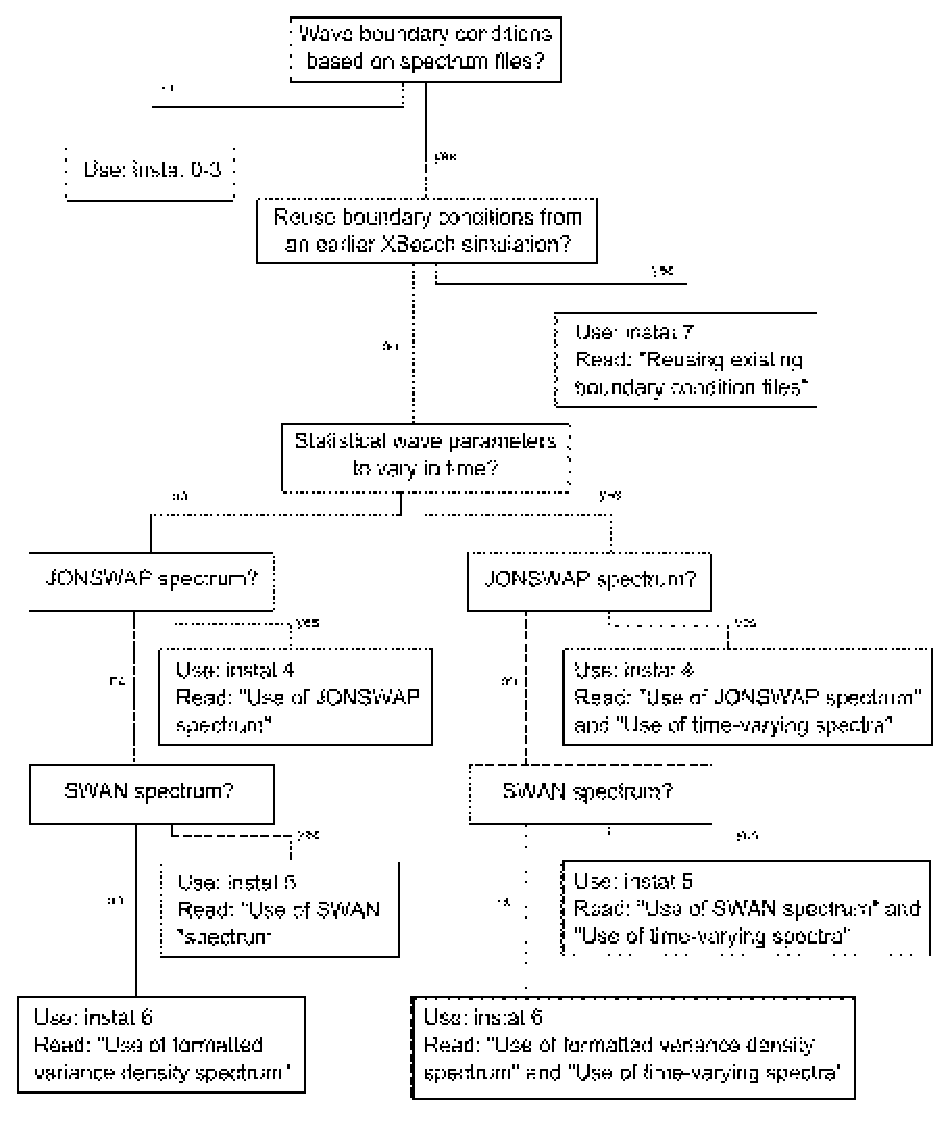
\includegraphics[width=0.6\textwidth]{image24}
  \caption{CityplaceReading guide}
  \label{fig:image24}
\end{figure}

\subsection{ Instat = 0 to 3. wave boundary condition parameters for non-spectral input}

\begin{tabular}{|p{0.5in}|p{1.1in}|p{0.4in}|p{0.5in}|p{0.5in}|p{0.3in}|p{0.7in}|} \hline 
keyword & description & default value & minimum value & maximum value & unit & remarks \\ \hline 
\textbf{dir0  } & mean wave direction (Nautical convention) & 270 & 180 & 360 & deg & instat=0-3 only \\ \hline 
\textbf{Hrms  } & rms wave height & 1 & 0 & 10 & m & instat=0-3 only \\ \hline 
\textbf{m     } & power in cos\^{}m directional distribution & 10 & 2 & 128 & - & instat=0-3 only \\ \hline 
\textbf{Tm01  } & spectral period & 10 & 1 & 20 & s & instat=0-3 only \\ \hline 
\textbf{Trep} & alternative keyword for representative period & 10 & 1 & 20 & s & instat=0-3 only; overrules value for Tm01 \\ \hline 
\textbf{Tlong } & long wave / wave group period & 80 & 20 & 300 & s & \textit{instat =} 1 only \\ \hline 
\textbf{taper    } & time to spin up wave boundary conditions & 100 & 1e-6 & 1000 & s & not for stationary waves \\ \hline 
\end{tabular}
\subsection{Instat = 4, spectral parameter input}

The new XBeach module allows the user to provide JONSWAP parameters from which XBeach computes a spectrum. To make use of this option, the user must specify \textit{`instat = 4'} in \textit{params.txt}. XBeach will then attempt to read JONSWAP parameters from a separate file specified by `\textit{bcfile =}' in \textit{params.txt}. The user must also state in \textit{params.txt} the required record length for the boundary condition file and the boundary condition file time step (keywords `\textit{rt =} ` and `\textit{dtbc =} ` respectively). If the record length (\textit{rt}) is less than the total simulation time, XBeach will reuse the boundary condition file until the simulation is completed. The boundary condition file time step should be small enough to accurately represent the bound long wave, but need not be as small as the time step used in XBeach, see \textit{Explanation of input/output}.

\begin{tabular}{|p{0.5in}|p{0.7in}|p{0.4in}|p{0.5in}|p{0.5in}|p{0.3in}|p{1.1in}|} \hline 
keyword & description & default value & minimum value & maximum value & unit & remarks \\ \hline 
\textbf{bcfile} & input file for spectral computations & - & - & - &  & file, with contents specified below \\ \hline 
\textbf{rt} & record length & 3600 & 1200 & 7200 & s &  \\ \hline 
\textbf{dtbc} & file time step & 0.5 & 0.1 & 2 & s &  \\ \hline 
\textbf{fcutoff} & low freq cutoff frequency for boundary conditions & 0 & 0 & 40 & Hz & for instat=4,5,6 \\ \hline 
\textbf{sprdthr} & threshold variance density above which spec dens are read in  & 0.08 & 0 & 1 & - & this is to reduce the spectral width \\ \hline 
\textbf{nspr} & set directional spreading long waves & 0 & 0 & 1 & - & 1 = bin all incoming long wave directions (instat 4+) in the centres of the short wave directional grid cells \\ \hline 
\textbf{trepfac} & Compute mean wave period over energy band: & 0.01 & 0 & 1 & - & par\%trepfac*maxval(Sf) for instat 4,5,6; converges to Tm01 for trepfac = 0.0  \\ \hline 
\textbf{random} & random generator & 1 & 0 & 1 &  & Random seed on \eqref{GrindEQ__1_} or off (0) \\ \hline 
\textbf{oldwbc} & old waveboundary condition & 0 & 0 & 1 & - & this value should stay at oldwbc=0. \\ \hline 
\end{tabular}

The contents of the file specified by `\textit{bcfile =}' in \textit{params.txt} is a list of \textit{keyword = value} combinations which determine the JONSWAP spectrum. These keywords are:

\begin{tabular}{|p{0.7in}|p{0.4in}|p{1.3in}|p{0.5in}|p{0.5in}|p{0.5in}|} \hline 
Keyword & Type & Description & Default & Minimum & Maximum \\ \hline 
`Hm0 = ' & real & H${}_{m0}$ of the wave spectrum, significant wave height [m] & 0.0 & 0.0 & 5.0 \\ \hline 
`fp = ' & real & Peak frequency of the wave spectrum [s${}^{-1}$] & 0.08 & 0.0625 & 0.4 \\ \hline 
`gammajsp = ' & real & Peak enhancement factor in the JONSWAP expression [-] & 3.3 & 1.0 & 5.0 \\ \hline 
`s = ' & real & Directional spreading coefficient, cosine law [-] & 10. & 1.0 & 1000. \\ \hline 
`mainang = ' & real & Main wave angle (in nautical terms) [${}^\circ$] & 270. & 180. & 360. \\ \hline 
`fnyq = ' & real & Highest frequency used to create JONSWAP spectrum [s${}^{-1}$] & 0.3 & 0.2 & 1.0 \\ \hline 
`dfj = ' & real & Step size frequency used to create JONSWAP spectrum [s${}^{-1}$] & fnyq/200 & fnyq/1000 & fnyq/20 \\ \hline 
\end{tabular}

All variables are optional. If no value is given, the default value is used. It is advised not to specify \textit{dfj} and allow XBeach to calculate the default value.

A typical input file contains the following:

\begin{tabular}{|p{1.5in}|p{1.5in}|p{1.5in}|} \hline 
XBeach Model Description and Manual & Z4175 & June 21, 20 \\ \hline 
&  &  \\ \hline 
\end{tabular}

D:\textbackslash mccall\textbackslash XBeach\textbackslash XBeach\_repository\textbackslash trunk\textbackslash doc\textbackslash xbeach\_manual.doc


\subsection{Instat = 5, SWAN spectrum input}

XBeach has been programmed to read standard SWAN 2D variance density or energy density output files (.sp2 files), as specified in the SWAN v40.51 manual. 

To make use of this option, the user must specify `\textit{instat =} 5' in \textit{params.txt}. XBeach will then read the SWAN output spectrum from a separate file specified by `\textit{bcfile =}' in \textit{params.txt}. The user must also state in \textit{params.txt} the required record length for the boundary condition file and the boundary condition file time step (keywords `\textit{rt =} ` and `\textit{dtbc =} ` respectively). If the record length (\textit{rt}) is less than the total simulation time, XBeach will reuse the boundary condition file until the simulation is completed. The boundary condition file time step should be small enough to accurately represent the bound long wave, but need not be as small as the time step used in XBeach, see \textit{Explanation of input/output.} For definitions, see above.

XBeach assumes the output of the SWAN file is in nautical terms. If the file is in Cartesian angles, the user must specify the angle in degrees to rotate the x-axis in SWAN to the x-axis in XBeach (in Cartesian terms). This value is specified in \textit{params.txt} after the keyword `\textit{dthetaS\_XB =}'. 

\begin{tabular}{|p{0.6in}|p{0.7in}|p{0.4in}|p{0.5in}|p{0.5in}|p{0.3in}|p{0.9in}|} \hline 
keyword & description & default value & minimum value & maximum value & unit & remarks \\ \hline 
\textbf{dthetaS\_XB} & conversion of angles between SWAN and XBeach & 0 & -360 & 360 & deg & If SWAN input is not in nautical degrees, dthetaS\_XB is the angle from SWAN x-axis to XBeach x-axis in cathesian degrees\newline        \\ \hline 
\end{tabular}

An example of a SWAN 2D output file is given below:

\begin{tabular}{|p{1.5in}|p{1.5in}|p{1.5in}|} \hline 
XBeach Model Description and Manual & Z4175 & June 21, 20 \\ \hline 
&  &  \\ \hline 
\end{tabular}

D:\textbackslash mccall\textbackslash XBeach\textbackslash XBeach\_repository\textbackslash trunk\textbackslash doc\textbackslash xbeach\_manual.doc


\subsection{ Instat = 6, Use of formatted variance density spectrum}

If the user has 2D spectrum information, but not in SWAN or JONSWAP form, the user can create a formatted spectrum file which can be read by XBeach. 

To make use of this option, the user must specify `\textit{instat =} 6' in \textit{params.txt}. XBeach will then attempt to read the formatted output spectrum from a separate file specified by `\textit{bcfile =}' in \textit{params.txt}. The user must also state in \textit{params.txt} the required record length for the boundary condition file and the boundary condition file time step (keywords `\textit{rt =} ` and `\textit{dtbc =} ` respectively). If the record length (\textit{rt}) is less than the total simulation time, XBeach will reuse the boundary condition file until the simulation is completed. The boundary condition file time step should be small enough to accurately represent the bound long wave, but need not be as small as the time step used in XBeach, see \textit{Explanation of input/output.}

The contents of the file specified by `\textit{bcfile =}' in \textit{params.txt} must follow a specified format. The information should be as follows:

\begin{enumerate}
\item  First line: number of frequencies (integer)

\item  Second line onwards: column with frequencies in Hz (each on a new line)

\item  Then: number of angles (integer)

\item  Then onwards: column with angles in degrees (each on a new line)

\item  Then per line: row of variance density in each direction, per frequency (i.e. first row corresponds to variance density per direction in the first frequency band, second row of the second frequency band, etc.).
\end{enumerate}

Note that the angles in the input file must be in the calculation coordinate system of XBeach, i.e. 0${}^\circ$ is in the direction of the x-axis, 90${}^\circ$ is in the direction of the y-axis. Also, the angles must be increasing.

An example of a formatted variance density file is given below:

\begin{tabular}{|p{1.5in}|p{1.5in}|p{1.5in}|} \hline 
XBeach Model Description and Manual & Z4175 & June 21, 20 \\ \hline 
&  &  \\ \hline 
\end{tabular}

D:\textbackslash mccall\textbackslash XBeach\textbackslash XBeach\_repository\textbackslash trunk\textbackslash doc\textbackslash xbeach\_manual.doc


\subsection{Instat =7, reusing existing boundary condition files}

If the user does not wish to recalculate boundary condition files or specifically wants to reuse the boundary condition files of another XBeach simulation, it is possible to do so. In this case the user should select `\textit{instat =} 7' in \textit{params.txt}. No further wave boundary condition data need be given in \textit{params.txt}. Obviously, the calculation grid should remain the same between runs, as the angles and number of grid points are embedded in the boundary condition files.

In order to use instat 7, the user should copy \textit{ebcflist.bcf} and \textit{qbcflist.bcf} to the current directory. Additionally, the user should also copy all files listed in \textit{ebcflist.bcf} and \textit{qbcflist.bcf}. Generally, these files have \textit{E\_} and \textit{q\_} prefixes.


\subsection{ Use of time-varying spectra}

The new XBeach module allows the user to specify time-varying wave spectra on the offshore boundary. This is done by feeding in several input data files such as those used for instat 4, 5 or 6, and specifying the duration for which these spectra should occur.

To make use of this option, the user must specify the instat value (4, 5 or 6) associated with the input data type for the wave boundary conditions. XBeach will then attempt to read a list of input data filenames from a separate file specified by `\textit{bcfile ='} in \textit{params.txt}. This keyword is the same keyword as used for non-time-varying spectra. In order for XBeach to differentiate between time-varying and non-time-varying wave spectra, the file must have the following format.

The first word in the file must be the keyword `FILELIST'. In the following lines, each line contains the duration of this wave spectrum condition in seconds (similar to `\textit{rt'} in \textit{params.txt}), the required time step in this boundary condition file in seconds (similar to `\textit{dtbf'} in \textit{params.txt}) and the name of the input data file used to generate these boundary conditions. The duration and boundary condition time step in this file overrules `\textit{rt'} and `\textit{dtbf'} in \textit{params.txt}. XBeach will now not reuse any boundary condition time series, so the user must ensure that the total record length is greater than or equal to the simulation time.

A typical input file contains the following:

\begin{tabular}{|p{1.5in}|p{1.5in}|p{1.5in}|} \hline 
XBeach Model Description and Manual & Z4175 & June 21, 20 \\ \hline 
&  &  \\ \hline 
\end{tabular}

D:\textbackslash mccall\textbackslash XBeach\textbackslash XBeach\_repository\textbackslash trunk\textbackslash doc\textbackslash xbeach\_manual.doc



Note: It is not possible to use a mix of JONSWAP, SWAN and Variance Density files. It is also not possible to vary \textit{dthetaS\_XB} between files in case of non-nautical SWAN output. 


\subsection{ Use of space-varying spectra}

XBeach allows users to specify multiple input wave spectra, or time series of wave spectra (see use of time-varying spectra) at separate locations on the offshore boundary. In order to apply varying spectra on the offshore boundary, the user must specify `\textit{wbcversion = 3'} and `\textit{nspectrumloc= }ns', in \textit{params.txt}, where \textit{ns} is the number of locations in which a spectrum is to be defined. By default the number of spectra is one.

If multiple spectra are applied, the wave boundary condition file specified by the parameter \textit{bcfile ='} in \textit{params.txt} must contain information about the locations of the input spectra. This is achieved by setting the first line in the boundary condition file to the word `LOCLIST'. This line should be followed by one line per input spectrum location containing the world x-coordinate and world y-coordinate of the location that the input spectrum should apply, and the name of the file containing spectral wave information for the input spectrum (i.e. a jonswap parameter file, swan file, or ``FILELIST'' file).

A typical input file for a run with three Jonswap spectra contains the following:

\begin{tabular}{|p{1.5in}|p{1.5in}|p{1.5in}|} \hline 
XBeach Model Description and Manual & Z4175 & June 21, 20 \\ \hline 
&  &  \\ \hline 
\end{tabular}

D:\textbackslash mccall\textbackslash XBeach\textbackslash XBeach\_repository\textbackslash trunk\textbackslash doc\textbackslash xbeach\_manual.doc



The manner in which a time series of short wave energy and bound long wave flux is calculated per offshore boundary point for spatially varying spectra is given in Section 2.3.1. The user is reminded that along the offshore boundary of the model, the wave energy, rather than the wave height, is interpolated linearly between input spectra without consideration of the physical aspects of the intermediate bathymetry. In cases with large gradients in wave energy, direction or period, the user should specify sufficient input spectra for the model to accurately represent changes in offshore wave conditions. 

When applying spatially varying spectra, the user should ensure that all input spectra are of the same type (specified by the keyword \textit{instat} in \textit{params.txt}) and the time-administration parameters (\textit{rt} and \textit{dtbc}) are the same for all input spectra. 
\subsection{ Instat = 8, boundary conditions for non-hydrostatic model }

XBeach can be ran as a non-hydrostatic model, which is essentially the nonlinear shallow water  equations with dispersion terms and without a wave-action driver. The boundary conditions are described in a separate chapter and are activated using instat=8


\subsection{ Instat = 9, no boundary condition }

\underbar{}

This is a simple ``no wave action'' boundary condition. It still allows for a tidal record to be specified, however through the zs0file parameter, see Chapter 5.9 below.
\subsection{ Instat = 40, sequence of stationary sea states }

\underbar{}

While instat=0 specifies one stationary sea state (stationary in the sense that there are no wave groups), it is also possible to specify a series of seastates, each with a duration. This is done through a file as

instat   = 40

bcfile   = jonswap1.txt

where the name of the bcfile is free, but the structure of the contents is not. It should contain lines with

Hm0, Tp, angle, gamma \eqref{GrindEQ__3_3_}, spreading, duration (s), timestep (=0.05)

Ie

0.7 8 90 3.3 5 1000 0.05

0.8 7 110 3.3 5 1000 0.05


\subsection{  Instat = 41, sequence of sea states to make time-varying wave groups }

This is an extension of instat=4. With instat = 41 it is possible to specify a sea state on the basis of which wave groups are imposed on the model for a certain duration, then specify another sea state and run wave groups again without having to stop the model. 

This condition is specified as

instat   = 41

bcfile   = jonswap1.txt

where the name of the file is free and the structure of the contents is as in instat = 40.


\subsection{ Notes on generation of boundary conditions}

At the start of the XBeach simulation, XBeach checks whether non-stationary varying wave boundary conditions are to be used. If this is the case, it next checks whether the \textit{wave spectrum} of the wave boundary conditions is to change over time, or remain constant. If the wave spectrum is to remain constant, XBeach will only read from one input file to generate wave boundary conditions. If the wave spectrum is to vary in time, XBeach reads from multiple files. 

Whether or not the wave spectrum of the boundary conditions changes over time, the XBeach module requires a record length during which the current wave spectral parameters are to apply. For the duration of the record length, boundary conditions are calculated at every boundary condition file time step. These time steps are not required to be the same as the time steps in the XBeach main program; XBeach will interpolate where necessary. The boundary condition time steps should therefore only be small enough to accurately describe the incoming bound long waves. The statistical data for the generation of the wave boundary conditions is read from user-specified files. At this stage the XBeach module can interpret SWAN 2D variance density output files and JONSWAP parameters. 

The beginning and end of the boundary condition file is tapered by the XBeach module. This is done to ensure smooth transitions from one boundary condition file to the next.

The combination of a large record length and a small time step lead to large demands on the system memory. If the memory requirement is too large, the user must choose to either enlarge the boundary condition time step, or to reduce the record length. In case of the latter, several boundary condition files can be generated and read sequentially. It is unwise however to reduce the record length too much, as then the transitions between the boundary condition files start to play an important role.

Every time the XBeach wave boundary condition module is run, it outputs data to the local directory. Metadata about the wave boundary conditions are stored in list files: \textit{ebcflist.bcf} and \textit{qbcflist.bcf}. The main XBeach program uses the list files to know how and when to read and generate boundary condition files. The actual incoming short-wave energy and long-wave mass flux data is stored in other files. These files have  \textit{E\_} and \textit{q\_} prefixes. The main XBeach program uses these files for the actual forcing along the offshore edge. 
\section{Flow input}

The bed friction is influenced by the dimensionless friction coefficient \textit{cf} or the dimensional \textit{C }value. These values are uniform and stationary.

The horizontal viscosity is first composed by adding an overall background viscosity \textit{nuh }and a viscosity depending on the roller dissipation, tuned by \textit{nuhfac}. In the alongshore direction the viscosity may be multiplied by a factor \textit{nuhv} to account for additional advective mixing.

\begin{tabular}{|p{0.5in}|p{0.8in}|p{0.5in}|p{0.5in}|p{0.5in}|p{0.4in}|p{0.6in}|} \hline 
keyword & description & default value & minimum value & maximum value & unit & remarks \\ \hline 
\textbf{cf      } & flow friction coefficient & 0.003 & 0 & 0.1 & - &  \\ \hline 
\textbf{C       } & Chezy coefficient & sqrt(g/cf)  & 20 & 100 & m${}^{1/2}$/s & alternative for cf, overrules cf if set \\ \hline 
\textbf{nuh     } & horizontal background viscosity & 0.15 & 0 & 1 & m2/s &  \\ \hline 
\textbf{nuhfac  } & viscosity coefficient for roller induced turbulent horizontal viscosity & 0 & 0 & 1 & - &  \\ \hline 
\textbf{nuhv    } & additional shear dispersion factor & 1 & 1 & 20 & - & svendsen and putrevu (1994) \\ \hline 
\textbf{smag} & Smagorinski & 1 & 0 & 1 &  &  \\ \hline 
\textbf{lat     } & latitude & 0 & 0 & 90 & deg N &  \\ \hline 
\textbf{omega} & angular velocity of earth  & 1/24 & 0 & 1 & 1/hour &  \\ \hline 
\end{tabular}
\section{Flow boundary conditions}

Flow boundary conditions need to be specified on all sides of the domain. We will differentiate between the offshore, lateral and landward boundaries. 

The \textit{carspan} keyword is useful when you want to specify timeseries of free long waves incident on the sea boundary. In that case use the file bc\textbackslash gen.ezs, specify the time in the first column, the long wave elevation in the second column and zero wave energy in the third column.

\begin{tabular}{|p{0.5in}|p{0.9in}|p{0.4in}|p{0.5in}|p{0.5in}|p{0.3in}|p{0.7in}|} \hline 
keyword & description & default value & minimum value & maximum value & unit & remarks \\ \hline 
\textbf{front    } & seaward boundary condition & 1 & 0 & 4 & - & see table below \\ \hline 
\textbf{ARC      } & active reflection compensation at seaward boundary & 1 & 0 & 1 & - & 0 = off, 1 = on \\ \hline 
\textbf{order   } & order of wave steering at seaward boundary & 2 & 1 & 2 & - & 1 = first order , 2 = second order  \\ \hline 
\textbf{carspan} & free long wave input & 0 & 0 & 1 & - & 0 = use cg (default); 1 = use sqrt(gh) in \textit{instat =} 3 for c\&g tests \\ \hline 
\textbf{} &  &  &  &  &  &  \\ \hline 
\textbf{back     } & bayside boundary condition & 2 & 0 & 3 & - & see table below \\ \hline 
\textbf{} &  &  &  &  &  &  \\ \hline 
\textbf{left     } & left lateral boundary condition & 0 & 0 & 1 & - & 0 = `neumann', \newline 1 = `wall' \\ \hline 
\textbf{right    } & right lateral boundary condition & 0 & 0 & 1 & - & 0 = 'neumann', 1 = `wall' \\ \hline 
\textbf{} &  &  &  &  &  &  \\ \hline 
\textbf{epsi    } & weighting factor between steady flow and particle velocity & 0 & 0 & 1 & - & obsolete \\ \hline 
\end{tabular}
\subsection{}

\begin{tabular}{|p{0.5in}|p{0.8in}|p{2.6in}|} \hline 
front & abbreviated name & description \\ \hline 
0 & abs1d & absorbing-generating (weakly-reflective) boundary in 1D \\ \hline 
1 & abs2d & same, in 2D (default setting) \\ \hline 
2 & wall & no flux wall \\ \hline 
3 & wlevel & water level specification (from file) \\ \hline 
4 & nonh\_1d & boundary condition for nonhydrostatic option \\ \hline 
\end{tabular}

\begin{tabular}{|p{0.5in}|p{0.8in}|p{2.6in}|} \hline 
\textbf{back} & abbreviated name & description \\ \hline 
0 & wall & no flux wall \\ \hline 
1 & abs1d & absorbing-generating (weakly-reflective) boundary in 1D \\ \hline 
2 & abs2d & same, in 2D (default setting) \\ \hline 
3 & wlevel & water level specification (from file) \\ \hline 
\end{tabular}


\subsection{ Time-varying tide/surge}

XBeach can take in up to four time-vary tidal signals to be applied to the four boundaries.  A time-varying water level signal is read into XBeach by \textit{readtide.f90}, which is called from \textit{XBeach.f90}. \textit{readtide} opens the specified file in par\%zs0file, and uses par\%tideloc (number of water level signal locations to be read in) and par\%tidelen (length of input signals) to format the file reading statements.  The par\%zs0file must follow the format with the first column being time and each subsequent column containing the water level signals.  As a note, the input signal will be interpolated to the local time step of the simulation; therefore the signals only need to be long enough and temporally-fine enough to resolve the water level phenomenon of interest (i.e. tide variations, surge event). The above parameters and file name are specified in \textit{params.txt}.  If par\%tideloc is equal to zero, \textit{readtide} is not utilized and a uniform water level is applied according to par\%zs0.      

There are now four options for handling the tidal and/or surge contribution to the boundaries:

\begin{enumerate}
\item  Uniform water level

\item  One time-varying water level signal

\item  Two time-varying water level signals, which requires point of application indication.

\item  Four time-varying water level signals
\end{enumerate}

The uniform water level is applied according to par\%zs0, as stated above. For par\%tideloc equal to 1, one water level signal is read and applied to the offshore boundary and par\%zs0 is applied to the land boundary.  If par\%tideloc is equal to 2, two water level signals are read by \textit{readtide}. par\%paulrevere is utilized to indicate the locations of application for the two signals.  For par\%paulrevere equal to 0, one tidal record is applied to both sea corners and one tidal record to both land corners, whereas if par\%paulrevere is equal to 1, the first tidal record is applied to the (x=1,y=1) sea corner and the second tidal record (third column) to the (x=1,y=N) sea corner. For par\%tideloc equal to 4, four tidal records are read. These four time-varying signals need to be in ordered columns going clockwise around the domain, with first column signal being applied to (x=1,y=1). Therefore, the columns must follow the order of: 1. (x=1,y=1), 2. (x=1,y=N), 3. (x=N,y=N), 4. (x=N,y=1).

The input signal(s) is(are) interpolated spatially along the boundaries for par\%tideloc is equal to 2 (if par\%paulrevere=2, and if par\%paulrevere=1 and no land mass blocks the flow between the land and sea boundaries) and higher. The spatial interpolation occurs initially in \textit{wave\_init}, and subsequently at every time step in \textit{flow\_bc}. The input signal(s) is(are) also interpolated to the local time step in \textit{flow\_bc}.  

\begin{tabular}{|p{0.6in}|p{1.0in}|p{0.4in}|p{0.5in}|p{0.5in}|p{0.3in}|p{0.5in}|} \hline 
keyword & description & default value & minimum value & maximum value & unit & remarks \\ \hline 
\textbf{zs01    } & initial water level & 0 & -5 & 5 & m &  \\ \hline 
\textbf{tideloc  } & number of input tidal time series & 0 & 0 & 4 & - &  \\ \hline 
\textbf{paulrevere  } & option of sea/sea corner or sea/land corner specification & 0 & 0 & 1 & - &  \\ \hline 
\end{tabular}
\section{Wind}

\begin{tabular}{|p{0.6in}|p{0.9in}|p{0.4in}|p{0.5in}|p{0.5in}|p{0.4in}|p{0.5in}|} \hline 
keyword & description & default value & minimum value & maximum value & unit & remarks \\ \hline 
\textbf{rhoa    } & air density & 1.25 & 1 & 2 & kg/m3 &  \\ \hline 
\textbf{Cd      } & wind drag coefficient & 0.002 & 0.0001 & 0.01 & - &  \\ \hline 
\textbf{windv   } & wind velocity & 0 & 0 & 200 & m/s &  \\ \hline 
\textbf{windth  } & wind direction (nautical convention) & 270 & -360 & 360 & deg & . \\ \hline 
\end{tabular}

The implementation of the wind stress in the momentum balance in XBeach is based upon the work of \citet{Ruessink2001}.  The wind field is specified by the following parameters in \textit{params.txt}:

\begin{enumerate}
\item  par\%windth, the wind direction (Nautical coordinates)

\item  par\%windv, the wind velocity specified in m/s

\item  par\%rhoa, the air density (default 1.25 kg/m${}^{3}$)

\item  par\%Cd, the air drag coefficient (default 0.002, but should be looked into for simulations with wind velocities exceeding 50 m/s)
\end{enumerate}

The input wind direction is converted to radians and Cartesian coordinates prior to use in the momentum balance. The wind contribution is computed as an additional term in the x and y momentum balances.


\section{Limiters}

Especially in very shallow water some processes need to be limited to avoid unrealistic behaviour. The parameters below can be adjusted by the user. Reducing \textit{gammax} will reduce wave heights in very shallow water, probably 2 is a reasonable value. \textit{hmin} prevents very strong return flows or high concentrations. \textit{eps} determines whether points are dry or wet and can be taken quite small. \textit{hwci} limits the computation of wave-current interaction in very shallow water where the procedure may not converge.

\begin{tabular}{|p{0.5in}|p{0.9in}|p{0.4in}|p{0.5in}|p{0.5in}|p{0.3in}|p{0.6in}|} \hline 
keyword & description & default value & minimum value & maximum value & unit & remarks \\ \hline 
\textbf{gammax} & maximum ratio Hrms/hh & 2 & 0.4 & 5 & - &  \\ \hline 
\textbf{hmin  } & threshold water depth for concentration and return flow & 0.05 & 0.001 & 1 & m &  \\ \hline 
\textbf{eps     } & threshold depth for drying and flooding & 0.005 & 0.001 & 0.1 & m &  \\ \hline 
\textbf{umin    } & threshold velocity upwind scheme & 0.0 & 0.0 & 5 & m/s &  \\ \hline 
\textbf{hwci} & depth below which wci is not applied & 0.1 & 0.0001 & 1 & m &  \\ \hline 
\end{tabular}
\section{Sediment transport}

\begin{tabular}{|p{0.6in}|p{0.9in}|p{0.5in}|p{0.5in}|p{0.6in}|p{0.3in}|p{0.6in}|} \hline 
\textbf{keyword} & description & default value & minimum value & maximum value & unit & remarks \\ \hline 
\textbf{waveform} & option for waveshape model & 1 & 1 & 1 & - & 1='ruessink\_vanrijn'\newline 2='vanthiel'  \\ \hline 
\textbf{form} & equilibrium sed. conc. formulation & 1 & 1 & 2 & - & 1 = `soulsby\_ vanrijn',  \newline 2 = \newline `vanthiel\_vanrijn'  \\ \hline 
\textbf{thetanum} & option to switch between central and upwind scheme & 1 & 0.5 & 1 & [-] & 1=upwind\newline 0.5=central \\ \hline 
\textbf{z0       } & zero flow velocity level in Soulsby van Rijn (1997) sed.conc. expression & 0.006 & 0.0001 & 0.05 & m &  \\ \hline 
\textbf{facsl    } & bed slope factor & 0 & 0 & 1.6 &  &  \\ \hline 
\textbf{BRfac} & Calibration factor surface slope & 1 & 0 & 1 &  &  \\ \hline 
\textbf{turb} & Equilibrium sediment concentration computation option & 2 & - & - & - & 0='none',\newline 1='wave\_averaged'\newline 2='bore\_averaged' \\ \hline 
\textbf{rhos     } & density of sediment (no pores) & 2650 & 2400 & 2800 & kg/m3 &  \\ \hline 
\textbf{por      } & porosity & 0.4 & 0.3 & 0.5 & - &  \\ \hline 
\textbf{smax} & max shields value for overwash & -1 & -1 & 3 & [-] &  \\ \hline 
\textbf{lws} & longwave stirring & 1 & 0 & 1 &  & 1 = on; 0 = off \\ \hline 
\textbf{sws} & shortwave stirring & 1 & 0 & 1 &  & 1 = on; 0 = off \\ \hline 
\textbf{tsfac} & max value for fall velocity & 0.1 & 0.01 & 1 & [-] &  \\ \hline 
\textbf{facua} & asymmetry transport & 0 & 0 & 1 & - &  \\ \hline 
\textbf{rfb} &  & 1 & 0 & 1 & - & ONLY IF FORM=2\newline \newline If rfb = 1 then maximum wave surface slope is fed back in roller energy balance; else rfb = par\%Beta     \\ \hline 
\end{tabular}


\section{Multiple sediment fractions and hard layers}

Keywords related to hard layers and sediment classes:

\begin{tabular}{|p{0.6in}|p{0.9in}|p{0.5in}|p{0.5in}|p{0.4in}|p{0.4in}|p{0.7in}|} \hline 
\textbf{struct    } & option for hard structures & 0 & 0 & 1 &  & 0 = no revetment, 1 = multiple sediment classes \\ \hline 
\textbf{ne\_layer} &  &  &  &  &  &  \\ \hline 
\textbf{ngd       } & number of sediment classes & 1 & 1 & 20 & - &  \\ \hline 
\textbf{nd        } & number of sediment class layers & 3 & 3 & 1000 & - &  \\ \hline 
\textbf{dzg1      \newline dzg2\newline dzg3} & thickness of sediment class layers & 0.1 & 0.01 & 1 & - &  \\ \hline 
\textbf{D50} & uniform D50 sediment diameter & 0.0002 & - & - & m &  \\ \hline 
\textbf{D90} & uniform D90 sediment diameter & 0.0003 & - & - & m &  \\ \hline 
\textbf{sedcal} & factor on sediment transport & 1 & - & - & - & advanced option, leave at sedcal=1 \\ \hline 
\textbf{ucrcal} & factor on critical velocity for erosion & 1 & - & - & - & advanced option, leave at ucrcal=1 \\ \hline 
\textbf{} &  &  &  &  &  &  \\ \hline 
\end{tabular}

NEEDS MORE EXPLANATION FOR MULTIPLE SEDIMENT FRACTIONS


\section{Morphological updating and avalanching}

\begin{tabular}{|p{0.6in}|p{1.0in}|p{0.4in}|p{0.5in}|p{0.5in}|p{0.3in}|p{0.5in}|} \hline 
keyword\textbf{} & description & default value & minimum value & maximum value & unit & remarks \\ \hline 
\textbf{morfac   } & morphological factor & 0 & 0 & 1000 & - &  \\ \hline 
\textbf{morstart } & start time of morphological updates & 120 & 0 & 10000 & s &  \\ \hline 
\textbf{morfacopt} & type of morfac updating & 1 & 0 & 1 &  & 1 = on; 0 = off \\ \hline 
\textbf{sourcesink} & morphological updating based on sediment transport gradients or source sink & 0 & 0 & 1 & - & 0 =  gradients \newline 1= source sink \\ \hline 
\textbf{wetslp   } &  critical avalanching slope under water & 0.3 & 0.1 & 1 & - &  \\ \hline 
\textbf{dryslp   } & critical avalanching slope above water & 1 & 0.1 & 2 & - &  \\ \hline 
\textbf{hswitch  } & water depth at interface from wetslp to dryslp & 0.1 & 0.01 & 1 &  &  \\ \hline 
\textbf{dzmax} &  & 0.05 & 0.00 & 1 &  &  \\ \hline 
\end{tabular}


\section{Groundwater}

In order to use the groundwater module in XBeach, a number of parameters have been added to \textit{params.txt}. The keywords, their type, default value and description are given below.

\begin{tabular}{|p{0.7in}|p{0.7in}|p{0.6in}|p{0.5in}|p{0.5in}|p{0.3in}|p{0.6in}|} \hline 
keyword\textbf{} & description & default value & minimum value & maximum value & unit & remarks \\ \hline 
\textbf{gwflow} & switch parameter & 0 & 0 & 1 & - & Turns the groundwater module on \eqref{GrindEQ__1_} or off \eqref{GrindEQ__2_} \\ \hline 
\textbf{kx} & The Darcy permeability coefficient of the aquifer in x-direction & 1E-4 & 1E-5 & 1E-2 & ms${}^{-1}$ &  \\ \hline 
\textbf{ky} & The Darcy permeability coefficient of the aquifer in y-direction & kx & 1E-5 & 1E-2 & ms${}^{-1}$ &  \\ \hline 
\textbf{kz} & The Darcy permeability coefficient of the aquifer in z-direction & kx & 1E-5 & 1E-2 & ms${}^{-1}$ &  \\ \hline 
\textbf{dwetlayer} & Thickness of the interaction layer $d_{wetlayer} $ & 0.2d0 & 0.01 & 1 & m &   \\ \hline 
\textbf{aquiferbot} & The bed level of the aquifer is set to the value of \textit{aquiferbot} across the \newline entire domain & minval(zb)-3.d0 & -100 & 100 & m &   \\ \hline 
\textbf{aquiferbotfile} & The initial bed level of the aquifer from file & - &  &  & - & This keyword overrides the \textit{aquiferbot} keyword \\ \hline 
\textbf{gw0} & The initial groundwater head  & 0.d0 & -5.0 & 5.0 & m & uniform over domain \\ \hline 
\textbf{gw0file} & The initial groundwater head from file  & - &  &  & - & This keyword overrides the \textit{gw0} keyword \\ \hline 
\textbf{} &  &  &  &  &  &  \\ \hline 
\textbf{} &  &  &  &  &  &  \\ \hline 
\end{tabular}


\paragraph{Example}

An example is given in which the groundwater module is used and the vertical permeability coefficient in the vertical is set differently to that in the horizontal. The initial bed level of the aquifer is read from a file and the initial groundwater head is set to a uniform value. Other parameters are kept at their default values.


\section{Drifters}

\textit{}

\begin{tabular}{|p{0.6in}|p{1.0in}|p{0.4in}|p{0.5in}|p{0.5in}|p{0.3in}|p{0.5in}|} \hline 
keyword\textbf{} & description & default value & minimum value & maximum value & unit & remarks \\ \hline 
\textbf{ndrifter} & number of drifters & 0 & 0 & 50 & - &  \\ \hline 
\textbf{drifterfile} & name of drifter file & - & - & - & - &  \\ \hline 
\end{tabular}


\section{Discharge boundaries (river input)}

\textit{}

\begin{tabular}{|p{1.0in}|p{0.6in}|p{0.4in}|p{0.5in}|p{0.5in}|p{0.3in}|p{0.6in}|} \hline 
keyword\textbf{} & description & default value & minimum value & maximum value & unit & remarks \\ \hline 
\textbf{disch\_loc\_file} & discharge locations file & - & - & - & - & see description \newline below \\ \hline 
\textbf{disch\_timeseries\_file} & discharge time series fiel & - & - & - &  & see description \newline below \\ \hline 
\end{tabular}

The contents of the discharge locations file are a number of records equal to the number of discharge boundary sections, with for each record four numbers:

\textit{X\_begin Y\_begin X\_end Y\_end}

\textit{}

These world coordinates must be chosen such that they are close to the desired boundary and enclose the cell centers of the cells that must be part of the boundary section.

In the discharge time series file, the first column is time in seconds; the next columns give the total discharge time series per section.


\section{Nonhydrostatic}

\begin{tabular}{|p{0.7in}|p{0.9in}|p{0.4in}|p{0.5in}|p{0.5in}|p{0.3in}|p{0.5in}|} \hline 
keyword\textbf{} & description & default value & minimum value & maximum value & unit & remarks \\ \hline 
\textbf{secorder} & second order corrections to advection/non-linear terms based on mcCormack scheme & 0 & 0 & 1 & - &  \\ \hline 
\textbf{solver\_maxit} & Maximum number of iterations in the linear SIP solver & 30 & 1 & 1000 &  &  \\ \hline 
\textbf{solver\_acc} & accuracy with respect to the right-hand side used & 0.005 & 0.00001 & 0.1 &  &  \\ \hline 
\textbf{solver\_urelax} & Underrelaxation parameter & 0.92 & 0.5 & 0.99 &  &  \\ \hline 
\textbf{solver} & Solver used to solve the linear system, 1=SIP, 2=TRIDIAG (only for 1d) & 1 & 0 & 2 &  &  \\ \hline 
\textbf{kdmin} & Minimum value of kd (pi/dx $>$ minkd ) & 0.0 & 0.0 & 0.05 &  &  \\ \hline 
\textbf{dispc} & Coefficient in front of the vertical pressure gradient & 1 & 0.1 & 2 &  &  \\ \hline 
\textbf{Topt} & Absolute period to optimize coefficient & 10 & 1 & 20 &  &  \\ \hline 
\textbf{} &  &  &  &  &  &  \\ \hline 
\textbf{} &  &  &  &  &  &  \\ \hline 
\textbf{} &  &  &  &  &  &  \\ \hline 
\textbf{} &  &  &  &  &  &  \\ \hline 
\textbf{} &  &  &  &  &  &  \\ \hline 
\textbf{} &  &  &  &  &  &  \\ \hline 
\textbf{} &  &  &  &  &  &  \\ \hline 
\end{tabular}
\section{Data types}

XBeach allows the user to choose between three types of output data: regular spatial output, time-averaged spatial output and point output. Of these three types, only the regular spatial output existed in previous versions of XBeach.

\begin{tabular}{|p{0.6in}|p{1.0in}|p{0.4in}|p{0.5in}|p{0.5in}|p{0.3in}|p{0.5in}|} \hline 
keyword\textbf{} & description & default value & minimum value & maximum value & unit & remarks \\ \hline 
\textbf{nglobalvar} & number of global output variables & -1 & -1 & 20 & - & see below \\ \hline 
\textbf{nmeanvar} & number of mean variables & 0 & 0 & 15 & - &  \\ \hline 
\textbf{npoints} & number of point output locations & 0 & 0 & 50 & - &  \\ \hline 
\textbf{nrugauge} & number of runup gauges & 0 & 0 & 50 & - &  \\ \hline 
\end{tabular}

If nglovalvar is set to `-1' then the standard output variables consist of 'H    ', 'zs   ', 'zs0  ', 'zb   ', 'hh   ', 'u    ', 'v    ', 'ue   ', 've   ', 'urms ', 'Fx   ',   'Fy   ', 'ccg  ', 'ceqsg', 'ceqbg', 'Susg ', 'Svsg ', 'E    ', 'R    ', 'D    ', 'DR   ' 
\subsection{ Regular spatial output}

Regular spatial output describes the instantaneous state of variables across the entire model domain at various points in time. In previous versions of XBeach, the program automatically generated regular spatial output of 20 variables. In the current version of XBeach, the user may determine how many and which variables are output. 

To make use of this option the user must specify the number of output variables required using the \textit{`nglobalvar='} keyword in \textit{params.txt}. The value of \textit{nglobalvar} is always integer. This line is immediately followed by the keywords of the required variables, one per line. Refer to the \textit{Variable keywords} section for a list of keywords. An example of the declaration of regular spatial output is given below.

\textit{Example of the declaration of regular spatial output variables}

Output files generated using this option are given the name \textit{keyword.dat}, for example \textit{zs.dat}. The only exception is that files containing information about the wave height of the short waves are called \textit{hrms.dat} instead of \textit{H.dat} to maintain backward compatibility.
\subsection{ Time-averaged spatial output}

This output describes the time-averaged state of variables across the entire model domain at various points in time. The period used to average the variables is selected by the user and is described in the section \textit{Choosing output times}. The user may determine how many and which variables are output. To make use of this option the user must specify the number of output variables required using the \textit{`nmeanvar='} keyword in \textit{params.txt}. The value of \textit{nmeanvar} is always integer. This line is immediately followed by the keywords of the required variables, one on each subsequent line. Refer to the \textit{Variable keywords} section for a list of keywords. This statement block may be made before or after the regular spatial output block. An example of the declaration of time-averaged spatial output is given below.


\section{Selecting output data types}

XBeach v12 allows the user to choose between three types of output data: regular spatial output, time-averaged spatial output and point output. Of these three types, only the regular spatial output existed in previous versions of XBeach.
\subsection{ Regular spatial output}

Regular spatial output describes the instantaneous state of variables across the entire model domain at various points in time. In previous versions of XBeach, the program automatically generated regular spatial output of 20 variables. In the current version of XBeach, the user may determine how many and which variables are output. 

To make use of this option the user must specify the number of output variables required using the \textit{`nglobalvar='} keyword in \textit{params.txt}. The value of \textit{nglobalvar} is always integer. This line is immediately followed by the keywords of the required variables, one per line. Refer to the \textit{Variable keywords} section for a list of keywords. An example of the declaration of regular spatial output is given below.

\textit{Example of the declaration of regular spatial output variables}

Output files generated using this option are given the name \textit{keyword.dat}, for example \textit{zs.dat}. The only exception is that files containing information about the wave height of the short waves are called \textit{hrms.dat} instead of \textit{H.dat} to maintain backward compatibility.
\subsection{ Time-averaged spatial output}

This output describes the time-averaged state of variables across the entire model domain at various points in time. The period used to average the variables is selected by the user and is described in the section \textit{Choosing output times}. The user may determine how many and which variables are output. To make use of this option the user must specify the number of output variables required using the \textit{`nmeanvar='} keyword in \textit{params.txt}. The value of \textit{nmeanvar} is always integer. This line is immediately followed by the keywords of the required variables, one on each subsequent line. Refer to the \textit{Variable keywords} section for a list of keywords. This statement block may be made before or after the regular spatial output block. An example of the declaration of time-averaged spatial output is given below.

\textit{Example of the declaration of time-averaged spatial output variables}

Output files generated using this option are given the name \textit{keyword\_mean.dat}, for example \textit{zs\_mean.dat}. 
\subsection{ Point output}

Point output allows the user to select one or more locations for which a time series of data is provided. This output type is divided into two classes: fixed point output and runup gauge output.
\subparagraph{ Fixed point output}

This output describes a time-series of a number of variables at one point in the model domain. To make use of this option, the user must specify the number of output locations using the \textit{`npoints='} keyword in \textit{params.txt}. The value of \textit{npoints} is always integer. This statement is always immediately followed by one line per output location describing the location coordinates, the number of output variables required at that location and the output variable keywords. The location coordinates are given separately as x-coordinate and y-coordinate, in world coordinates. XBeach will link the output location to the nearest computational point. The number of required variables is integer. Variables are stated using their respective variable keywords, see the \textit{Variable keywords} section. Each keyword, including the last keyword, must be followed by a number symbol (\#).This statement block may be made before or after any other output option block. All variables will be outputted for all points. 

An example is given below in which two output locations are defined. The first point is located on the offshore boundary (x-coordinate = 0.0) and somewhere in the middle of the model domain in y-direction (y-coordinate = 800.0). This location has two output variables, \textit{u} and \textit{v}. The second point is located on the lateral boundary (y-coordinate = 1600.0) and somewhere in the middle of the domain in x-direction (x-coordinate = 2000.0). This location has four output variables, \textit{H}, \textit{zs}, \textit{zb} and \textit{D}. 


\subparagraph{ Runup gauge output}

This output describes a time-series of a number of variables at the waterline. In this case XBeach scans in a x-directional transect defined by the user to find the last wet point before shore (defined as the first dry point in a transect). Output information is recorded for this point. This is particularly useful to keep track of runup levels in cross shore transects. 

The definition of runup gauges is similar to the definition of fixed point output. To specify runup gauges, the user should specify the number of runup gauges using the \textit{'nrugauge='} keyword in \textit{params.txt}. The value of \textit{nrugauge} is always integer. This statement is always immediately followed by one line per output location describing the location coordinates, the number of output variables required at that location and the output variable keywords. The location coordinates are given separately as x-coordinate and y-coordinate, in world coordinates. XBeach will link the output location to the nearest computational grid row. The number of required variables is integer. Variables are stated using their respective variable keywords, see the \textit{Variable keywords} section. Each keyword, including the last keyword, must be followed by a number symbol (\#).This statement block may be made before or after any other output option block. All variables will be used for each point.
\subparagraph{ Point output file structure}

All data corresponding to point locations will be stored in files called \textit{pointxxx.dat} in the case of fixed point data and \textit{rugauxxx.dat} in the case of runup gauge data. In the filenames \textit{xxx} represents a number between 001 and 999, corresponding to the order in which the points are declared in \textit{params.txt}. The data files contain one row per output time step. The first position on each row is the time at which the output is given. The subsequent positions in the row are the values of the variables at the given point at that given moment. The order of the variables is the same as the order in which they are defined for that point in \textit{params.txt}. 
\subsection{ Cross-sections}

NOT YET IMPLEMENTED
\subsection{ Default values}

If no output information is given with respect to the numbers and types of output, XBeach assumes the user requires only the original 20 regular spatial output types. The default number of time-averaged output variables and point output locations is zero.
\section{Choosing output times}

The user may determine the output times for regular spatial output variables, time averaged spatial variables and point location variables individually. Runup gauge output and fixed point output are given at the same points in time. For all three types of output the user may choose to either state a fixed interval time at which output is given, or supply an additional file containing times at which output should be given. 
\subsection{ Output at fixed intervals}

In this case the user should define a point in time (in seconds) after the start of the simulation at which the first output is generated. The user can do this by using the \textit{`tstart='} keyword in \textit{params.txt}. All output that is being generated at fixed intervals uses \textit{tstart} as their base. The interval for regular global output is given by the \textit{`tintg='} keyword in \textit{params.txt}. The keywords for the interval of time-averaged global output and point output are \textit{`tintm='} and \textit{`tintp='} respectively. Note that \textit{tintg}, \textit{tintm} and \textit{tintp} supersede the older \textit{tint} parameter. An example of the definition of fixed intervals is given below.

\textit{Example of the declaration of fixed interval output times}

In the case of regular global output and point output, the first output is given at \textit{tstart}. In the case of time-averaged global variables, the first output is given at \textit{tstart+tintm}. This output represents the average condition over the interval between \textit{tstart} and \textit{tstart+tintm}. 
\subsection{ Output times defined by external file}

The user is given the option to have output at a set of points in time that are not separated by regular intervals. In this case the user must supply an additional file for each output type (regular, time-averaged or point). The user specifies the name of the output time series file for regular spatial output using the \textit{`tsglobal='} keyword in \textit{params.txt}. The keywords for time series files for time-averaged output and point output are \textit{'tsmean='} and \textit{`tspoint='} respectively. All time series files must contain on the first line the number of output times (integer) followed by every output time (in seconds after the start of the simulation) on a new line. An example of the definition of varying output time intervals is given below. An example of the contents of one of the time series definition files is given in the second example below.

\textit{Example of the declaration of varying output time intervals}

\textit{Example of an output time series definition file (in the previous example this could be timeseries1.txt)}

In the case of regular global output and point output, the first output is given at the first stated point in time. In the case of time-averaged global variables, the first output is given at the second stated point in time. This output represents the average condition over the interval between first and second stated point in time. Subsequent averaging is made over every interval.
\subsection{ Combinations of fixed interval and external files}

The user is allowed to define certain types of output using fixed intervals and others using external files. The use of an external file supersedes the use of fixed intervals. Note that \textit{tstart} will only apply to output of fixed interval type. An example of mixing fixed and varying output time intervals is given below.

\textit{Example of the declaration of fixed and varying output time intervals}
\subsection{ Default values}

The default value of \textit{tintg} is one second. If \textit{tintp} or \textit{tintm} is not stated, but output is declared (\textit{npoints}, \textit{nrugauge} or \textit{nmeanvar} is stated larger than zero), XBeach assumes the same output interval as \textit{tintg}. XBeach v12 has been designed to be backward compatible with older versions. Therefore if \textit{tint} is defined, this replaces the default value of \textit{tintg}. 


\section{NetCDF -- CF output }

The netcdf output will be stored in the file xboutput.nc. Netcdf output is generated using the keyword \textit{outputformat}. 

An example of the layout of the netcdf file is given below. One thing to note is the different time dimensions. This is because of the different resolutions of point output and global output. The temporal unit can be specified in the params.txt file using the keyword \textit{tunits}. This unit does not affect calculations and is only used for output. 




\section{Reading output files in Matlab}

Various functions have been developed to help users read XBeach output in Matlab. The following script can be used to gather information about the XBeach output before reading the output.

\textit{Matlab function to extract output metadata}

Regular spatial output and time-averaged output can then be read using the following function.

\textit{Matlab function to read spatial output variables}

To read point data the following function can be used.

\textit{Matlab function to read point output variables}








\section{Output variable keywords}

All variables in spaceparams.tmpl can be defined as output. 



real*8  2  x  s\%nx+1 s\%ny+1  d    [m]        x-coord. comp. grid (positive shoreward, perp. to coastline)

real*8  2  y  s\%nx+1 s\%ny+1  d    [m]        y-coord. comp. grid

real*8  1  xz s\%nx+1 d    [m]        x-coord. comp. grid (positive shoreward, perp. to coastline)

real*8  1  yz s\%ny+1 d    [m]        y-coord. comp. grid

real*8  1  xu s\%nx+1  d    [m]        x-coord. in u points

real*8  1  yv s\%ny+1  d    [m]        y-coord. in v points

real*8  2  xw s\%nx+1 s\%ny+1  d    [m]        world x-coordinates

real*8  2  yw s\%nx+1 s\%ny+1  d    [m]        world y-coordinates

real*8  0  dx   b    [m]        grid size x-direction

real*8  0  dy   b    [m]        grid size y-direction

real*8  0  xori b    [m]        x-origin of grid in world coordinates

real*8  0  yori b    [m]        y-origin of grid in world coordinates

real*8  0  alfa b    [rad]      (deg on input) angle of grid w.r.t. East

real*8  0  posdwn b  [-]        depths defined positive downwards \eqref{GrindEQ__1_} or upwards(-1)

real*8  0  thetamin b  [rad]      minimum angle of computational wave grid (carth. in rad)

real*8  0  thetamax b  [rad]      minimum angle of computational wave grid (carth. in rad)

integer 0  nx     b  [-]        local number of grid cells x-direction

integer 0  ny     b  [-]        local number of grid cells y-direction

real*8  2  zb     s\%nx+1 s\%ny+1 d  [m]        bed level

real*8  2  zb0    s\%nx+1 s\%ny+1 d  [m]        initial bed level

real*8  1  theta  s\%ntheta b  [rad]      wave angles directional distribution w.r.t. comp. x-axis

integer 0  ntheta b  [-]        number of wave direction bins

real*8  0  dtheta b  [rad]      wave direction bin size

real*8  0  theta0 b  [rad]      mean incident wave angle

real*8  1  cxsth  s\%ntheta b  [-]        cos(theta)

real*8  1  sxnth  s\%ntheta b  [-]        sin(theta)

real*8  2  thetamean s\%nx+1 s\%ny+1 d  [rad]      mean wave angle

real*8  2  Fx     s\%nx+1 s\%ny+1 d  [N/m2]     wave force x-direction

real*8  2  Fy     s\%nx+1 s\%ny+1 d  [N/m2]     wave force y-direction

real*8  2  Sxy    s\%nx+1 s\%ny+1 d  [N/m]      radiation stress

real*8  2  Syy    s\%nx+1 s\%ny+1 d  [N/m]      radiation stress

real*8  2  Sxx    s\%nx+1 s\%ny+1 d  [N/m]      radiation stress

real*8  2  n      s\%nx+1 s\%ny+1 d  [-]        ratio group velocity/wave celerity

real*8  2  H      s\%nx+1 s\%ny+1 d  [m]        wave height 

real*8  3  cgx    s\%nx+1 s\%ny+1 s\%ntheta d  [m/s]      group velocity x-direction

real*8  3  cgy    s\%nx+1 s\%ny+1 s\%ntheta d  [m/s]      group velocity y-direction

real*8  3  cx     s\%nx+1 s\%ny+1 s\%ntheta d  [m/s]      wave celerity x-direction

real*8  3  cy     s\%nx+1 s\%ny+1 s\%ntheta d  [m/s]      wave celerity y-direction

real*8  3  ctheta s\%nx+1 s\%ny+1 s\%ntheta d  [rad/s]    wave celerity theta-direction (refraction)

real*8  3  ee     s\%nx+1 s\%ny+1 s\%ntheta d  [J/m2/rad] directionally distributed wave energy

real*8  3  thet   s\%nx+1 s\%ny+1 s\%ntheta d  [rad]      wave angles  

real*8  3  costhet s\%nx+1 s\%ny+1 s\%ntheta d   [-]        cos of wave angles  

real*8  3  sinthet s\%nx+1 s\%ny+1 s\%ntheta d  [-]        sin of wave angles  

real*8  3  sigt   s\%nx+1 s\%ny+1 s\%ntheta d  [rad/s]    relative frequency 

real*8  3  rr     s\%nx+1 s\%ny+1 s\%ntheta d  [J/m2/rad] directionally distributed roller energy

real*8  2  k      s\%nx+1 s\%ny+1 d  [rad/m]    wave number

real*8  2  c      s\%nx+1 s\%ny+1 d  [m/s]      wave celerity

real*8  2  cg     s\%nx+1 s\%ny+1 d  [m/s]      group velocity

real*8  2  sigm   s\%nx+1 s\%ny+1 d  [rad/s]    mean frequency

real*8  2  wm     s\%nx+1 s\%ny+1 d  [rad/s]    mean abs frequency

real*8  2  hh     s\%nx+1 s\%ny+1 d  [m]        water depth

real*8  2  zs     s\%nx+1 s\%ny+1 d  [m]        water level

real*8  2  zs0    s\%nx+1 s\%ny+1 d  [m]        water level due to tide alone

real*8  1  tideinpt par\%tidelen b  [s]        input time of input tidal signal

real*8  2  tideinpz par\%tidelen par\%tideloc b  [m]        input tidal signal

real*8  1  windinpt par\%windlen b  [s]        input time of input wind signal

real*8  1  windvel  par\%windlen b  [m/s]        input wind velocity

real*8  1  winddir  par\%windlen b  [deg nautical]        input wind direction

real*8  0  windvnow b              [m/s]      uniform wind velocity current time

real*8  0  winddirnow b            [m/s]      uniform wind direction current time

real*8  2  dzsdt  s\%nx+1 s\%ny+1 d  [m/s]      rate of change water level

real*8  2  dzsdx  s\%nx+1 s\%ny+1 d  [m/s]      water surface gradient in x-direction

real*8  2  dzsdy  s\%nx+1 s\%ny+1 d  [m/s]      water surface gradient in y-direction

real*8  2  dzbdx  s\%nx+1 s\%ny+1 d  [-]        bed level gradient in x-direction

real*8  2  dzbdy  s\%nx+1 s\%ny+1 d  [-]        bed level gradient in y-direction

real*8  2  dzbdt  s\%nx+1 s\%ny+1 d  [m/s]      rate of change bed level 

real*8  2  uu     s\%nx+1 s\%ny+1 d  [m/s]      (GLM) x-velocity in u-points

real*8  2  vv     s\%nx+1 s\%ny+1 d  [m/s]      (GLM) y-velocity in v-points

real*8  2  qx     s\%nx+1 s\%ny+1 d  [m2/s]     x-discharge in u-points

real*8  2  qy     s\%nx+1 s\%ny+1 d  [m2/s]     y-discharge in u-points

real*8  2  sedero s\%nx+1 s\%ny+1 d  [m]        cum. sedimentation/erosion

real*8  2  dcbdx   s\%nx+1 s\%ny+1 d  [kg/m3/m]  bed concentration gradient x-dir.

real*8  2  dcbdy   s\%nx+1 s\%ny+1 d  [kg/m3/m]  bed concentration gradient y-dir.

real*8  2  dcsdx   s\%nx+1 s\%ny+1 d  [kg/m3/m]  suspended concentration gradient x-dir.

real*8  2  dcsdy   s\%nx+1 s\%ny+1 d  [kg/m3/m]  suspended concentration gradient y-dir.

real*8  2  ui     s\%nx+1 s\%ny+1 d  [m/s]      incident bound wave velocity

real*8  2  E      s\%nx+1 s\%ny+1 d  [Nm/m2]    wave energy

real*8  2  R      s\%nx+1 s\%ny+1 d  [Nm/m2]    roller energy

real*8  2  urms   s\%nx+1 s\%ny+1 d  [m/s]      orbital velocity

real*8  2  D      s\%nx+1 s\%ny+1 d  [W/m2]     dissipation

real*8  2  Qb     s\%nx+1 s\%ny+1 d  [-]        fraction breaking waves

real*8  2  ust    s\%nx+1 s\%ny+1 d  [m/s]      Stokes drift

real*8  2  tm     s\%nx+1 s\%ny+1 d  [rad]      mean wave direction

real*8  2  ueu    s\%nx+1 s\%ny+1 d  [m/s]      Eulerian mean velocity x-dir.

real*8  2  vev    s\%nx+1 s\%ny+1 d  [m/s]      Eulerian mean velocity y-dir.

real*8  2  vmagu  s\%nx+1 s\%ny+1 d  [m/s]      (GLM) velocity magnitude u-points

real*8  2  vmageu s\%nx+1 s\%ny+1 d  [m/s]      (GLM) velocity magnitude u-points

real*8  2  vmagv  s\%nx+1 s\%ny+1 d  [m/s]      (GLM) velocity magnitude v-points

real*8  2  vmagev s\%nx+1 s\%ny+1 d  [m/s]      (GLM) velocity magnitude v-points

real*8  2  u      s\%nx+1 s\%ny+1 d  [m/s]      (GLM) x-velocity cell centre (for output)

real*8  2  v      s\%nx+1 s\%ny+1 d  [m/s]      (GLM) y-velocity cell centre (for output)

real*8  2  ue     s\%nx+1 s\%ny+1 d  [m/s]      Eulerian mean x-velocity cell centre (for output)

real*8  2  ve     s\%nx+1 s\%ny+1 d  [m/s]      Eulerian mean y-velocity cell centre (for output)

real*8  2  hold   s\%nx+1 s\%ny+1 d  [m]        water depth previous time step

integer 2  wetu   s\%nx+1 s\%ny+1 d  [-]        mask wet/dry u-points

integer 2  wetv   s\%nx+1 s\%ny+1 d  [-]        mask wet/dry v-points

integer 2  wetz   s\%nx+1 s\%ny+1 d  [-]        mask wet/dry eta-points

real*8  2  hu     s\%nx+1 s\%ny+1 d  [m]        water depth in u-points

real*8  2  hv     s\%nx+1 s\%ny+1 d  [m]        water depth in v-points

real*8  2  hum    s\%nx+1 s\%ny+1 d  [m]        water depth in u-points

real*8  2  hvm    s\%nx+1 s\%ny+1 d  [m]        water depth in v-points

real*8  2  vmag   s\%nx+1 s\%ny+1 d  [m/s]      velocity magnitude in cell centre

real*8  3  ccg    s\%nx+1 s\%ny+1 par\%ngd d  [m3/m3]    depth-averaged suspended concentration for each sediment fraction

real*8  3  ccbg   s\%nx+1 s\%ny+1 par\%ngd d  [m3/m3]    depth-averaged bed concentration for each sediment fraction

real*8  2  uwf    s\%nx+1 s\%ny+1 d  [m/s]      x-comp. Stokes drift

real*8  2  vwf    s\%nx+1 s\%ny+1 d  [m/s]      y-comp. Stokes drift

real*8  2  ustr   s\%nx+1 s\%ny+1 d  [m/s]      return flow due to roller

real*8  2  usd    s\%nx+1 s\%ny+1 d  [m/s]      return flow due to roller after breaker delay

real*8  1  bi     s\%ny+1 d  [m]        incoming bound long wave

real*8  2  DR     s\%nx+1 s\%ny+1 d  [W/m2]     roller energy dissipation

real*8  2  umean  2 s\%ny+1 2  [m/s]      longterm mean velocity at bnds in x-direction

real*8  2  vmean  2 s\%ny+1 2  [m/s]      longterm mean velocity at bnds in y-direction

integer 0  vardx  b  [-]        0 = uniform grid size, 1 = variable grid size

real*8  2  vu     s\%nx+1 s\%ny+1 d  [m/s]      y velocity in u points          

real*8  2  uv     s\%nx+1 s\%ny+1 d  [m/s]          x velocity in v points

real*8  1  D50    par\%ngd b  [m]        D50 grain diameters for all sediment classses

real*8  1  D90    par\%ngd b  [m]        D90 grain diameters for all sediment classses

real*8  1  sedcal par\%ngd b  [-]        equilibrium sediment concentartion factor for each sediment class

real*8  1  ucrcal par\%ngd b  [-]        calibration factor for u critical for each sediment class

real*8  3  Tsg    s\%nx+1 s\%ny+1 par\%ngd d  [s]        sediment response time for each sediment class

real*8  3  Susg    s\%nx+1 s\%ny+1 par\%ngd d  [m2/s]    suspended sediment transport x-dir. for each sediment class (excluding pores)

real*8  3  Svsg    s\%nx+1 s\%ny+1 par\%ngd d  [m2/s]    suspended sediment transport y-dir. for each sediment class (excluding pores)

real*8  3  Subg    s\%nx+1 s\%ny+1 par\%ngd d  [m2/s]    bed sediment transport x-dir. for each sediment class (excluding pores)

real*8  3  Svbg    s\%nx+1 s\%ny+1 par\%ngd d  [m2/s]    bed sediment transport y-dir. for each sediment class (excluding pores)

real*8  3  ceqbg s\%nx+1 s\%ny+1 par\%ngd d  [m3/m3]    depth-averaged bed equilibrium concentration for each sediment class

real*8  3  ceqsg s\%nx+1 s\%ny+1 par\%ngd d  [m3/m3]    depth-averaged suspended equilibrium concentration for each sediment class

real*8  2  ua     s\%nx+1 s\%ny+1 d  [m/s]      time averaged flow velocity due to wave assymetry

real*8  2  BR     s\%nx+1 s\%ny+1 d  [-]        maximum wave surface slope used in roller dissipation formulation

real*8  2  kb s\%nx+1 s\%ny+1 d  [m\^{}2/s\^{}2]  near bed turbulence intensity due to depth induces breaking

real*8  2  Tbore s\%nx+1 s\%ny+1 d  [s]        wave period interval associated with breaking induced turbulence

real*8  2  dzav   s\%nx+1 s\%ny+1 d  [m]        total bed level change due to avalanching

real*8  2  maxzs  s\%nx+1 s\%ny+1 d  [m]        maximum elevation in simulation  

real*8  2  minzs  s\%nx+1 s\%ny+1 d  [m]        minimum elevation in simulation 

real*8  2  L1     s\%nx+1 s\%ny+1 d  for subroutine dispersion

real*8  2  Sk s\%nx+1 s\%ny+1 d  [-] skewness of short waves

real*8  2  As s\%nx+1 s\%ny+1 d  [-] asymmetry of short waves

!      real*8  2  Fimpact s\%nx+1 s\%ny+1 d ! [N/m\^{}2]    Force on dune face

real*8  2  gwhead   s\%nx+1 s\%ny+1 d  [m] groundwater head (differs from gwlevel)

real*8  2  gwlevel  s\%nx+1 s\%ny+1 d  [m] groundwater table (min(zb,gwhead))

real*8  2  gwheight s\%nx+1 s\%ny+1 d  [m] vertical size of aquifer through which groundwater can flow

real*8  2  gwbottom s\%nx+1 s\%ny+1 d  [m] level of the bottom of the aquifer

real*8  2  gwu      s\%nx+1 s\%ny+1 d  [m/s] groundwater flow in x-direction

real*8  2  gwv      s\%nx+1 s\%ny+1 d  [m/s] groundwater flow in y-direction

real*8  2  gww      s\%nx+1 s\%ny+1 d  [m/s] groundwater flow in z-direction (interaction between surface and ground water)

real*8  2  dinfil   s\%nx+1 s\%ny+1 d  [m] Infiltration layer depth used in quasi-vertical flow model for groundwater

real*8  2  gw0back  2      s\%ny+1 2  [m] boundary condition back boundary for groundwater head

real*8  2  kturb    s\%nx+1 s\%ny+1 d  [m\^{}2/s\^{}2]  depth averaged turbulence intensity due to long wave breaking

real*8  3  ero      s\%nx+1 s\%ny+1 par\%ngd d  [m/s] bed erosion rate per fraction

real*8  3  depo\_im     s\%nx+1 s\%ny+1 par\%ngd d  [m/s] implicit bed deposition rate per fraction

real*8  3  depo\_ex     s\%nx+1 s\%ny+1 par\%ngd d  [m/s] explicit bed deposition rate per fraction

integer 2  nd       s\%nx+1 s\%ny+1 d  [-]  number of bed layers (can be different for each computational cell)

real*8  4  pbbed    s\%nx+1 s\%ny+1 max(par\%nd,2) par\%ngd d [-] NO DESCRIPTION

real*8  3  dzbed    s\%nx+1 s\%ny+1 max(par\%nd,2) d [-] NO DESCRIPTION

real*8  2  z0bed    s\%nx+1 s\%ny+1 d  [-] NO DESCRIPTION

real*8  2  ureps     s\%nx+1 s\%ny+1 d [m/s] representative flow velocitie for sediment advection and diffusion in x-direction

real*8  2  vreps     s\%nx+1 s\%ny+1 d  [m/s] representative flow velocitie for sediment advection and diffusion in y-direction

real*8  2  urepb     s\%nx+1 s\%ny+1 d [m/s] representative flow velocitie for sediment advection and diffusion in x-direction

real*8  2  vrepb     s\%nx+1 s\%ny+1 d [m/s] representative flow velocitie for sediment advection and diffusion in y-direction

real*8  2  umwci     s\%nx+1 s\%ny+1 d  [m/s]    u-velocity (time-averaged) for wci

real*8  2  rolthick s\%nx+1 s\%ny+1 d  [m]  long wave roller thickness

real*8  2  vmwci     s\%nx+1 s\%ny+1 d  [m/s]    v-velocity (time-averaged) for wci

real*8  2  zswci     s\%nx+1 s\%ny+1 d  [m]    waterlevel (time-averaged) for wci

real*8  2  pres      s\%nx+1 s\%ny+1 d  [m\^{}2/s\^{}2] normalized dynamic pressure

real*8  2  wb        s\%nx+1 s\%ny+1 d  [m/s]     vertical velocity at the bottom

real*8  2  ws        s\%nx+1 s\%ny+1 d  [m/s]     vertical velocity at the free surface

real*8  2  taubx     s\%nx+1 s\%ny+1 d  [N/m\^{}2]   x-component of bed shear stress

real*8  2  tauby     s\%nx+1 s\%ny+1 d  [N/m\^{}2]   y-component of bed shear stress

real*8  2  Df        s\%nx+1 s\%ny+1 d  [W/m\^{}2]   dissipation rate due to bed friction

real*8  2  Dp        s\%nx+1 s\%ny+1 d  [W/m\^{}2]   dissipation rate in the swash due to transformation of kinetic wave energy to potential wave energy

real*8  2  Sutot     s\%nx+1 s\%ny+1 d  [m2/s]   Sediment transport integrated over bed load and suspended and for all sediment grains

real*8  2  Svtot     s\%nx+1 s\%ny+1 d  [m2/s]   Sediment transport integrated over bed load and suspended and for all sediment grains

real*8  2  cctot     s\%nx+1 s\%ny+1 d  [m3/m3]   Sediment concentration integrated over bed load and suspended and for all sediment grains

real*8  2  wi        2      s\%ny+1 2  [m/s]   Vertical velocity at boundary due to (short) waves2

real*8  2  zi        2      s\%ny+1 2  [m]     Surface elevation at boundary due to (short) waves

real*8  2  nuh       s\%nx+1 s\%ny+1 d  [m2/s] horizontal viscosity coefficient 

real*8  2  cf        s\%nx+1 s\%ny+1 d  [-] Friction coefficient flow

real*8  2  D50top    s\%nx+1 s\%ny+1 d  [-] Friction coefficient flow

real*8  2  D90top    s\%nx+1 s\%ny+1 d  [-] Friction coefficient flow

real*8  2  structdepth    s\%nx+1 s\%ny+1 d  [m] Depth of structure in relation to instantaneous bed level




\section{Example params.txt file}

The following example shows a partial \textit{params.txt} file in which all three types of output are specified.

\textit{Example of a shortened params.txt file with various output options}

%%% Local Variables: 
%%% mode: latex
%%% TeX-master: "xbeach_manual"
%%% End: 
